%************************************************
\chapter{Introduction}\label{ch:introduction}
%************************************************
\section{Structure of the Milky Way}\label{sec:intro}
\subsection{Milky Way as a disc galaxy}
\begin{figure}[t]
	\begin{center}
		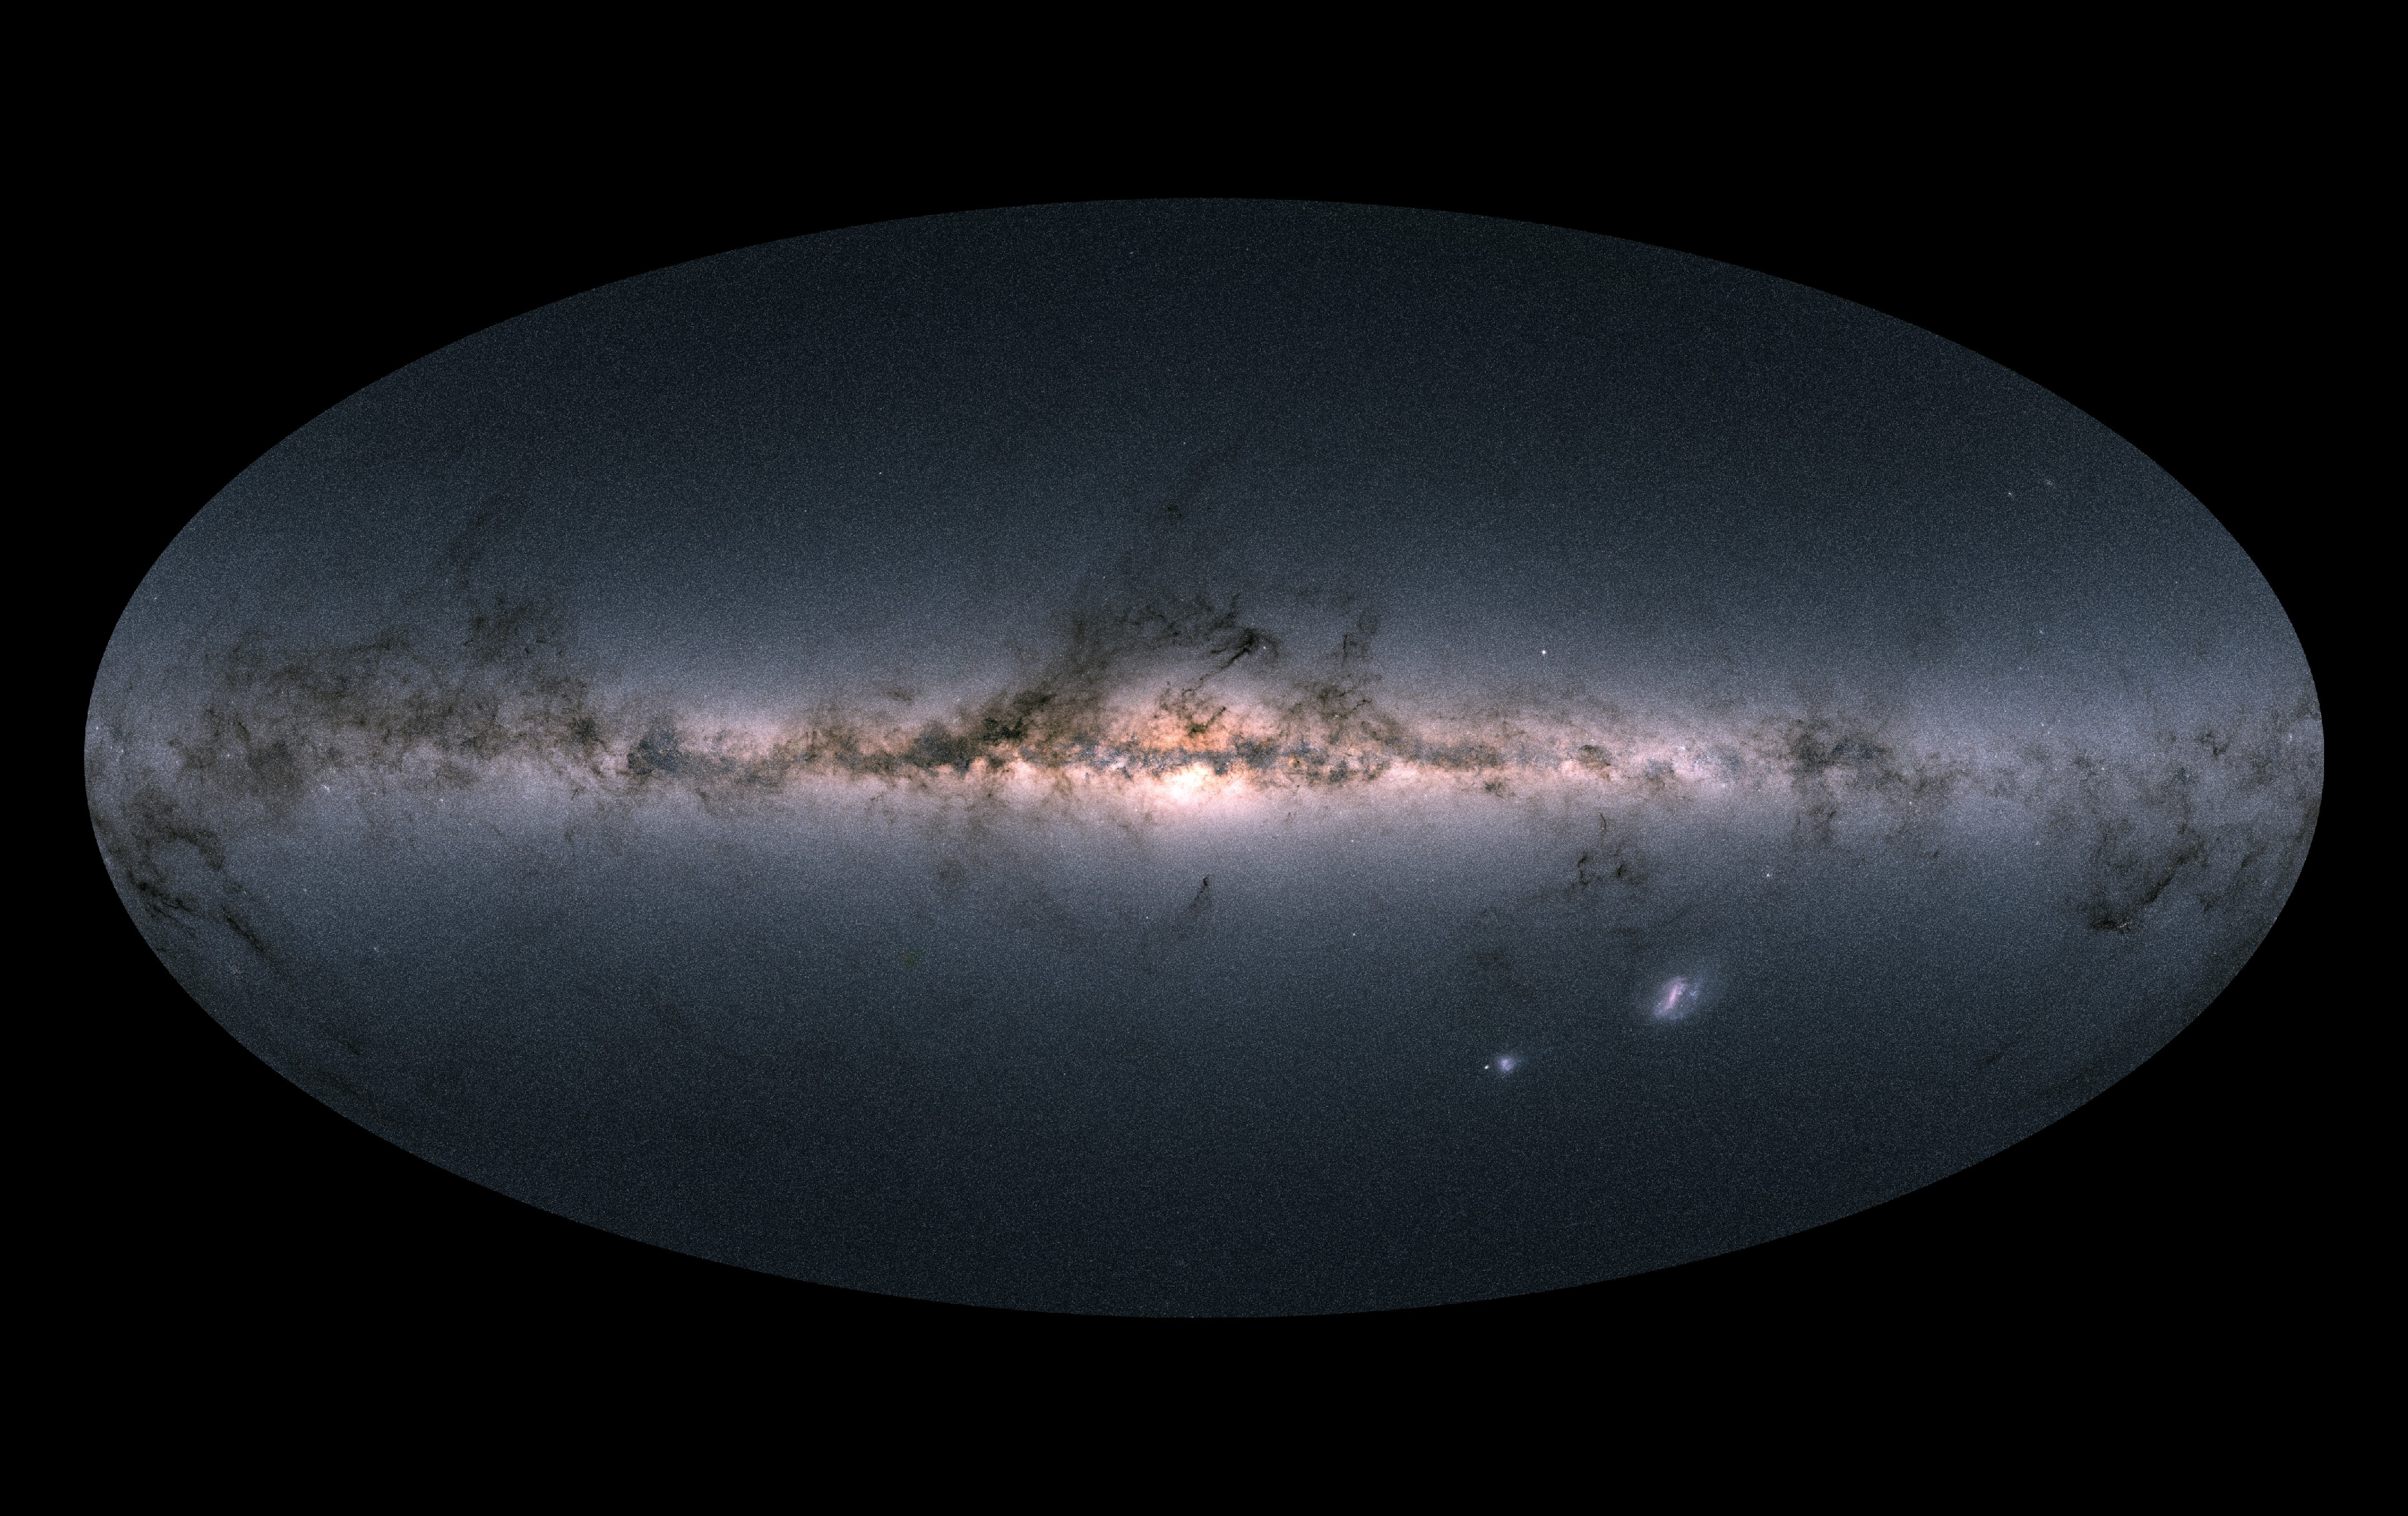
\includegraphics[width=0.8\linewidth]{figs/Gaia_s_sky_in_colour.pdf}
		\caption[Optical image of the MW obtained by the \textit{Gaia} satellite]{Optical image of the MW obtained by the \textit{Gaia} satellite. Credit: ESA/Gaia/DPAC.}\label{fig:gaia_sky}
	\end{center}
\end{figure}
The \ac{MW} has fascinated us throughout human history.
Fig.~\ref{fig:gaia_sky} displays an all-sky image of the \ac{MW} obtained by the \textit{Gaia} satellite. It is a portrait of our home galaxy as seen from the solar system.
Although we cannot observe our galaxy from the outside, we know that it is a barred spiral galaxy. This section provides a brief  history of our understanding of the \ac{MW}'s structure and summarises our current knowledge.
Throughout this section, we refer to the following books and papers: \citet{1998gaas.book.....B}, \citet{2008gady.book.....B}, \citet{2016ARA&A..54..529B}, \citet{2017gra..book.....S}, \citet{Ginga2} and \citet{vanderKruit2019}.

William Herschel was a pioneer in mapping the \ac{MW} based on scientific observations and measurements \citep{1785RSPT...75..213H}. He estimated the shape of the \ac{MW} by counting the number of stars at over 600 different directions in the sky assisted by his sister Caroline. The number count is proportional to $D^3$, where $D$ is the distance to the edge. This estimation relied on the following assumptions: (1) stars are uniformly distributed in the \ac{MW}, (2) all stars have the same intrinsic luminosity and (3) the telescope is powerful enough to see through the \ac{MW} to its edge.
Fig.~\ref{fig:mw_herschel} presents the estimated map of the \ac{MW}, which corresponds to the edge-on slice of the \ac{MW} disc. The large star near the centre of the map indicates the position of the Sun.
It is surprising that Herschel could estimate the flat disc-like shape of the \ac{MW} with such a simple method and rough assumptions although he mapped the Sun at the wrong place.
\begin{figure}[t]
	\begin{center}
		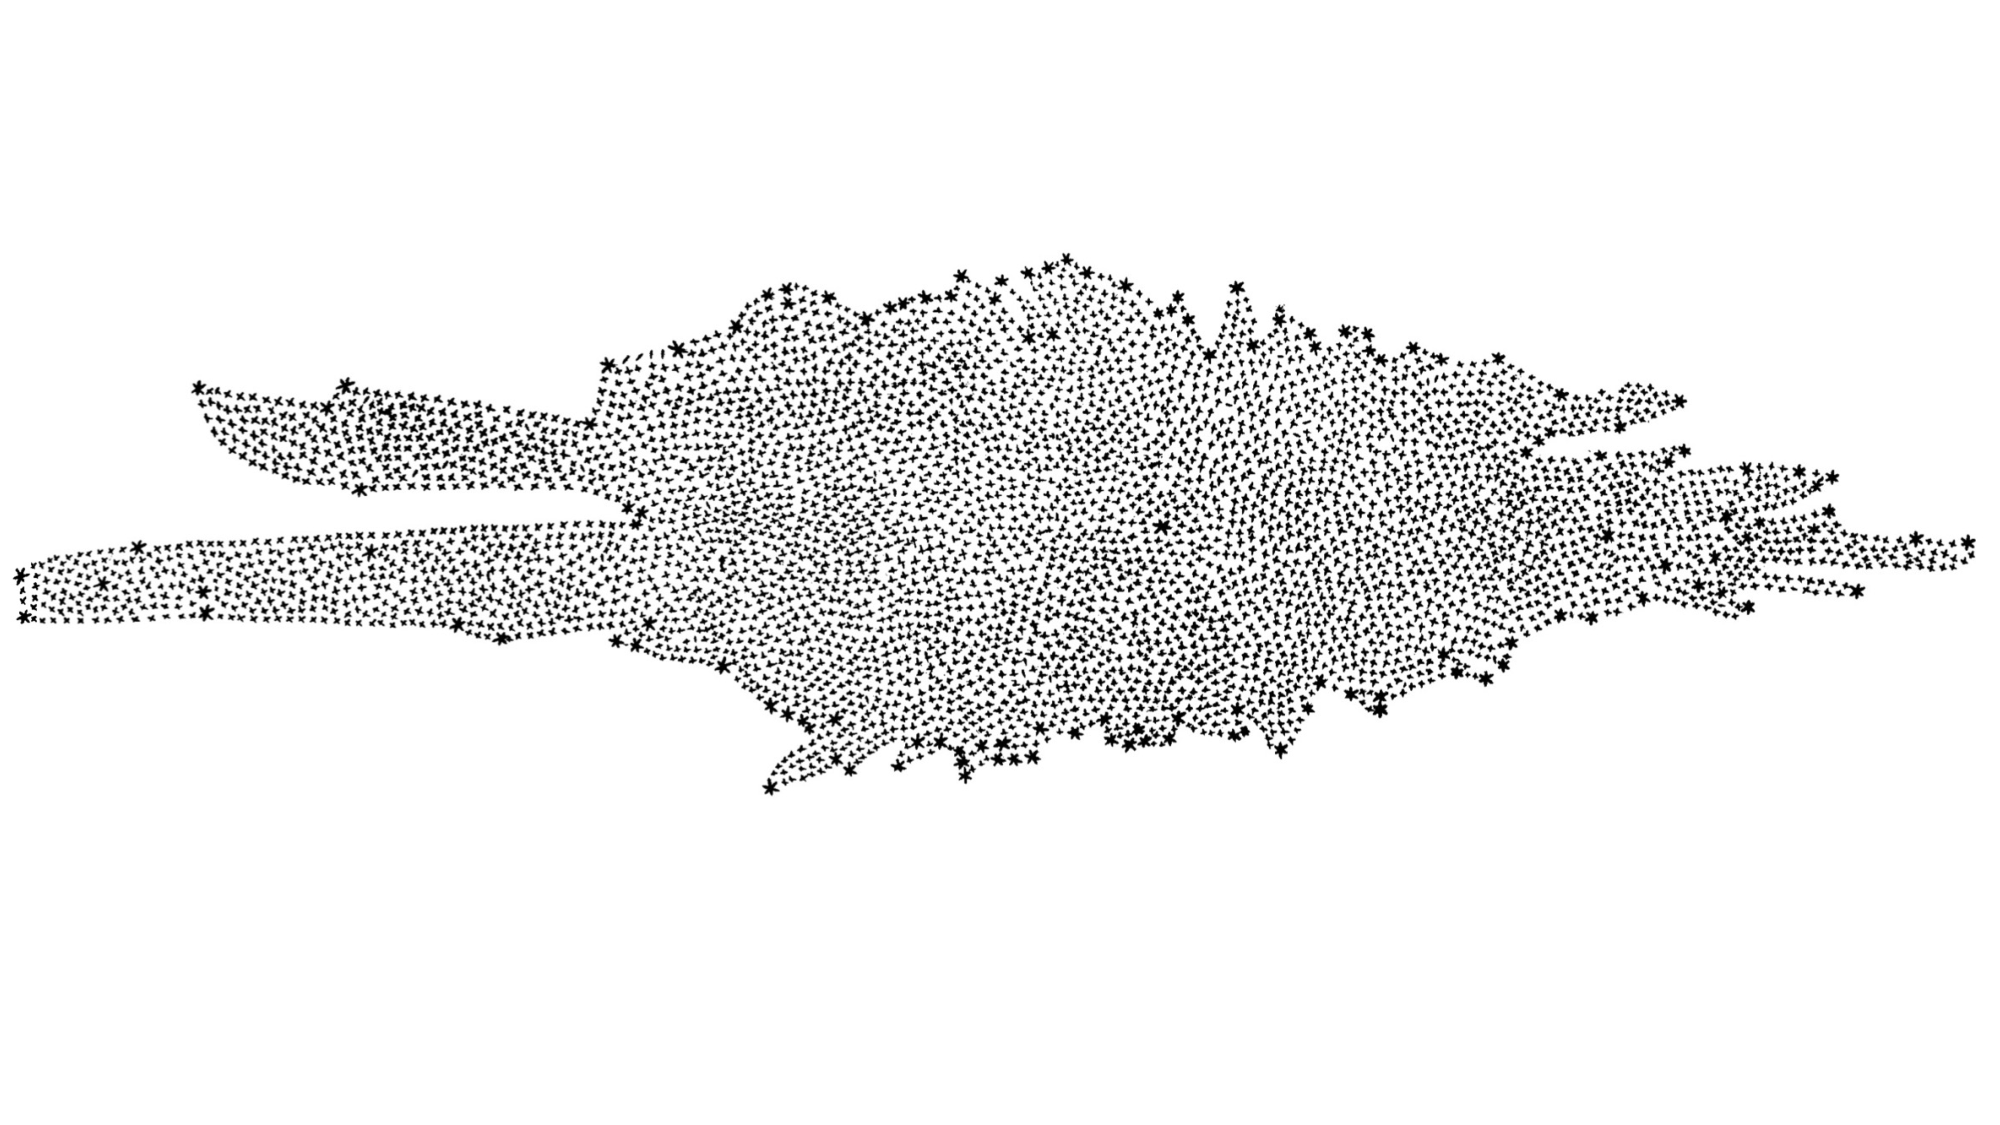
\includegraphics[width=\linewidth, trim={0cm 1cm 0cm 1cm}]{figs/Herschel_MW.pdf}
		\caption[Herschel's MW map]{Herschel's \ac{MW} map. The large star near the centre of the map indicates the position of the Sun. This figure is made from a copy of \citet{1785RSPT...75..213H} available at \url{https://www.jstor.org/stable/106755}.}
		\label{fig:mw_herschel}
	\end{center}
\end{figure}

